\documentclass[12pt]{article}

% Use packages %
\usepackage{graphicx, courier, amsmath, amssymb, amscd, amsfonts, mathtools, bm, esint, leftidx, extarrows, latexsym, relsize, color, tikz, comment, stmaryrd, float}
\usepackage[obeyspaces]{url}% http://ctan.org/pkg/url

% Set length %
\setlength{\textwidth}{160mm}
\setlength{\textheight}{235mm}
\setlength{\oddsidemargin}{-0mm}
\setlength{\topmargin}{-10mm}

% Define h-bar %
\newsavebox{\myhbar}
\savebox{\myhbar}{$\hbar$}
\renewcommand*{\hbar}{\mathalpha{\usebox{\myhbar}}}

% Chinese input %
%\usepackage{xeCJK} 
%\setCJKmainfont{微軟正黑體}
%\usepackage[T1]{fontenc}
%\makeatletter

% Equation number %
%\@addtoreset{equation}{section} 
%\renewcommand\theequation{{\thesection}.{\arabic{equation}}}
%\makeatletter 

% Helper Command %
\newcommand{\argmin}{\operatornamewithlimits{argmin}}
\newcommand{\rmnum}[1]{\romannumeral #1} 
\newcommand{\Rmnum}[1]{\expandafter\@slowromancap\romannumeral #1@}
\newcommand{\overbar}[1]{\mkern 1.5mu\overline{\mkern-1.5mu#1\mkern-1.5mu}\mkern 1.5mu}
\makeatother
\newcommand*{\QEDA}{\hfill\ensuremath{\blacksquare}}
\newcommand*{\QEDB}{\hfill\ensuremath{\square}}
\newcommand*{\BmVert}{\bigm\vert}
\newcommand{\bigslant}[2]{{\raisebox{.2em}{$#1$}\left/\raisebox{-.2em}{$#2$}\right.}}
\newcommand{\Nelements}[3]{\left\{ #1, ~ #2, \ldots, ~ #3 \right\}}
\newcommand{\CBrackets}[1]{\left\{#1\right\}}
\newcommand{\SBrackets}[1]{\left[#1\right]}
\newcommand{\BooBrackets}[1]{\left\llbracket#1\right\rrbracket}
\newcommand{\ParTh}[1]{\left(#1\right)}
\newcommand{\Ceil}[1]{\left\lceil#1\right\rceil}
\newcommand{\Floor}[1]{\left\lfloor#1\right\rfloor}
\newcommand{\BF}[1]{{\bf#1}}
\newcommand{\Inverse}[1]{{#1}^{-1}}
\newcommand{\Generator}[1]{\left\langle#1\right\rangle}
\newcommand{\AbsVal}[1]{\left|#1\right|}
\newcommand{\VecAbsVal}[1]{\left\|#1\right\|}
\newcommand{\BSlash}[2]{\left.#1\middle\backslash#2\right.}
\newcommand{\Divide}[2]{\left.#1\middle/#2\right.}
\newcommand{\SciNum}[2]{#1\times{10}^{#2}}
\newcommand{\Matrix}[2]{\ParTh{\begin{array}{#1}#2\end{array}}}
\newcommand{\MatrixTwo}[4]{\ParTh{\begin{array}{cc}{#1}&{#2}\\{#3}&{#4}\end{array}}}
\newcommand{\MatrixNByN}[1]{\Matrix{cccc}{{#1}_{11} & {#1}_{12} & \cdots & {#1}_{1n} \\ {#1}_{21} & {#1}_{22} & \cdots & {#1}_{2n} \\ \vdots & \vdots & \ddots & \vdots \\ {#1}_{n1} & {#1}_{n2} & \cdots & {#1}_{nn}}}
\newcommand{\ndiv}{\hspace{-4pt}\not|\hspace{2pt}}
\newcommand{\eqdef}{\xlongequal{\text{def}}}%
\newcount\arrowcount
\newcommand\arrows[1]{\global\arrowcount#1 \ifnum\arrowcount>0
\begin{matrix}\expandafter\nextarrow\fi}
\newcommand\nextarrow[1]{\global\advance\arrowcount-1 \ifx\relax#1\relax\else \xrightarrow{#1}\fi\ifnum\arrowcount=0 \end{matrix}\else\\\expandafter\nextarrow\fi}
\newcommand{\horrule}[1]{\rule{\linewidth}{#1}}

% Tikz settings %
\usetikzlibrary{shapes,arrows}
\tikzstyle{decision} = [diamond, draw, fill=white!20, text width=4.5em, text badly centered, node distance=3cm, inner sep=0pt]
\tikzstyle{block}    = [rectangle, draw, fill=white!20, text width=8em, text centered, rounded corners, minimum height=4em]
\tikzstyle{point}    = [fill = white!20, minimum size=0.5cm]
\tikzstyle{line}     = [draw, -latex']
\tikzstyle{mapsto}   = [draw, |->]
\tikzstyle{cloud}    = [draw, ellipse,fill=red!20, node distance=3cm, minimum height=2em]

\begin{document}

\baselineskip 6.5mm
\setlength{\parindent}{0pt}
\title{ 
\normalfont \normalsize 
\horrule{0.5pt} \\[0.4cm]
\huge { \Huge Machine Learning \\ \large Answer Sheet for Homework 8}\\
\horrule{2pt} \\ [0.5cm]
}
\author{ { \Large Da-Min HUANG } \\
{\small R04942045} \\
{\small\textit{Graduate Institute of Communication Engineering, National Taiwan University}}
}
\date{January 20, 2016}
%\allowdisplaybreaks[4]
\maketitle

\subsection*{Problem 1}

\begin{enumerate}
	\item Forward:
	\begin{align}
	\ParTh{A+1}\times B+\ParTh{B+1}\times1=\ParTh{A+2}B+1
	\end{align}
	\item Backward:
	
	$\delta^{\ParTh{L}}_1=-2\ParTh{y_n-s^{\ParTh{L}}_1}x^{\ParTh{L-1}}_i$ counts and
	\begin{align}
	\dfrac{\partial e_n}{\partial w^{\ParTh{\ell}}_{ij}}=\delta^{\ParTh{\ell}}_jx^{\ParTh{\ell-1}}_i\text{ for }0\leq i\leq d^{\ParTh{\ell-1}}\text{ and }1\leq j\leq d^{\ParTh{\ell}}
	\end{align}
	with
	\begin{align}
	\delta^{\ParTh{\ell}}_j=\sum_{k}\ParTh{\delta^{\ParTh{\ell+1}}_k}\ParTh{w^{\ParTh{\ell+1}}_{jk}}\ParTh{\tanh^\prime\ParTh{s^{\ell}_j}}
	\end{align}
	So one backward counts
	\begin{align}
	\underbrace{\ParTh{B+1}\times1}_{\text{output layer}}+\underbrace{B\times\ParTh{A+1}}_{\text{hidden layer}}+\underbrace{B}_{\text{hidden layer }\delta^{\ParTh{\ell}}_j}=\ParTh{A+3}B+1
	\end{align}
\end{enumerate}
Hence, total number of operations required in a single iteration of backpropagation is
\begin{align}
\ParTh{\ParTh{A+2}B+1}+\ParTh{\ParTh{A+3}B+1}=\ParTh{2A+5}B+2
\end{align}

\QEDB

\horrule{0.5pt}

\subsection*{Problem 2}

Suppose we have $k$ hidden layers, which means $L=k+1$, with $d^{\ParTh{1}}$, $d^{\ParTh{2}}$,$\ldots$, $d^{\ParTh{k}}$ units ($x^{\ParTh{\ell}}_0$ is not counted here) in each layer. The number of total weights is
\begin{align}
\sum_{i=0}^{k-1}\ParTh{d^{\ParTh{i}}+1}d^{\ParTh{i+1}}+\ParTh{d^{\ParTh{k}}+1}\times1=\sum_{i=0}^{k-1}d^{\ParTh{i}}d^{\ParTh{i+1}}+\sum_{j=1}^{k}d^{\ParTh{j}}+\ParTh{d^{\ParTh{k}}+1}\coloneqq N_w
\end{align}
with
\begin{align}
\sum_{j=1}^{k}\ParTh{d^{\ParTh{j}}+1}=\ParTh{\sum_{j=1}^{k}d^{\ParTh{j}}}+k=36\text{ and }d^{\ParTh{0}}=9
\end{align}
So we have
\begin{align}
N_w=\ParTh{37-k}+9d^{\ParTh{1}}+\ParTh{\sum_{i=1}^{k-1}d^{\ParTh{i}}d^{\ParTh{i+1}}}+d^{\ParTh{k}}
\end{align}
Since $d^{\ParTh{\ell}}\geq1$ for $0\leq\ell\leq k+1$, so we have $1\leq k\leq18$.

\underline{Claim}: $k=18$ minimizes $N_w$.

\underline{Proof of Claim}:

If $k=18$, we have 2 units in each hidden layer (one is $x^{\ParTh{\ell}}_0$, not counted in $d^{\ParTh{\ell}}$), so
\begin{align}
\left.N_w\right|_{k=18}=\ParTh{37-18}+9\times1+\ParTh{\sum_{i=1}^{17}1\times1}+1=46
\end{align}
\begin{comment}
If $k=17$, consider the following cases
\begin{enumerate}
	\item Put two units of original $d^{\ParTh{18}}$ (include $x^{\ParTh{18}}_0$) in some hidden layer. If in the last hidden layer, we have
	\begin{align}
	\left.N_w\right|_{k=17}=\ParTh{37-17}+9\times1+\ParTh{\sum_{i=1}^{15}1\times1+1\times\ParTh{1+2}}+3=50>\left.N_w\right|_{k=18}
	\end{align}
	If in some $d^{\ParTh{\ell}}$ with $2\leq\ell\leq16$ (if $\ell=1$ then $N_w$ will be added more then 9), we have
	\begin{align}
	\left.N_w\right|_{k=17}=\ParTh{37-17}+9\times1+\ParTh{\sum_{i=1}^{14}1\times1+1\times3+3\times1}+2=51>\left.N_w\right|_{k=18}
	\end{align}
	\item Put one unit in some hidden layer and one in some other hidden layer.  W.L.O.G., put the one unit in $d^{\ParTh{17}}$ and one in $d^{\ParTh{16}}$, we have
	\begin{align}
	\left.N_w\right|_{k=17}=\ParTh{37-17}+9\times1+\ParTh{\sum_{i=1}^{14}1\times1+1\times2+2\times2}+2=50>\left.N_w\right|_{k=18}
	\end{align}
\end{enumerate}
\end{comment}
If $k=18-m$, $m\in\mathbb{N}$ and $1\leq m\leq17$, we have
\begin{align}
\left.N_w\right|_{k=18-m}&=\ParTh{19+m}+9d^{\prime\ParTh{1}}+\ParTh{\sum_{i=1}^{17-m}d^{\prime\ParTh{i}}d^{\prime\ParTh{i+1}}}+d^{\prime\ParTh{18-m}}\\
\label{2-1}
&\geq\ParTh{19+m}+9+\ParTh{17-m}+1\\
&=19+9+17+1=\left.N_w\right|_{k=18}
\end{align}
where $d^{\prime\ParTh{\ell}}$ is the new number of each hidden layer if $k=18-m$ and (\ref{2-1}) holds due to $d^{\prime\ParTh{i}}d^{\prime\ParTh{i+1}}\geq1$ and $d^{\prime\ParTh{i}}\geq1$, $\forall i$ (by definition).

Hence, we have $N_w\geq46$.

\QEDB

\horrule{0.5pt}

\subsection*{Problem 3}

Following the setting of Problem 2.

\underline{Claim}: $k=2$ with $21$ units (not included $x^{\ParTh{1}}_0$) in $d^{\ParTh{1}}$ and $13$ units (not included $x^{\ParTh{2}}_0$) in $d^{\ParTh{2}}$ maxmizes $N_w$.

\underline{Proof of Claim}:

If $k=2$ with $21$ units (not included $x^{\ParTh{1}}_0$) in $d^{\ParTh{1}}$ and $13$ units (not included $x^{\ParTh{2}}_0$) in $d^{\ParTh{2}}$, we have
\begin{align}
\left.N_w\right|_{k=2}=\ParTh{37-2}+9\times21+\ParTh{21\times13}+13=510
\end{align}
Consider following cases,
\begin{enumerate}
	\item If $k=2$ with $34-m$ units (not included $x^{\ParTh{1}}_0$) in $d^{\ParTh{1}}$ and $m$ units (not included $x^{\ParTh{2}}_0$) in $d^{\ParTh{2}}$, where $m\in\mathbb{N}$ and $1\leq m\leq33$, we have
	\begin{align}
	\left.N_w\right|_{k=2}=\ParTh{37-2}+9\times\ParTh{34-m}+\ParTh{\ParTh{34-m}\times m}+m=-\ParTh{m-13}^2+510
	\end{align}
	Hence, $m=13$ maximize $\left.N_w\right|_{k=2}$.
	\item If $k=1$.
	\begin{align}
	\left.N_w\right|_{k=1}=\ParTh{37-1}+9\times35+35=386<510
	\end{align}
	\item If $k=3$ with $33-n_1-n_2$ units (not included $x^{\ParTh{1}}_0$) in $d^{\ParTh{1}}$, $n_1$ units (not included $x^{\ParTh{2}}_0$) in $d^{\ParTh{2}}$ and $n_2$ units (not included $x^{\ParTh{3}}_0$) in $d^{\ParTh{3}}$, where $n_1,n_2\in\mathbb{N}$ and $1\leq n_1,n_2\leq31$, we have
	\begin{align}
	\left.N_w\right|_{k=3}&=\ParTh{37-3}+9\times\ParTh{33-n_1-n_2}+\ParTh{\ParTh{33-n_1-n_2}\times n_1+n_1\times n_2}+n_2\\
	&=-\ParTh{n_1-12}^2-8n_2+475\leq-8n_2+475\leq467<510
	\end{align}
	We can see that this results in 9-20-12-1-1 neural network, which is equal to grab one neuron (and one constant neuron) from 9-21-13-1 neural network to create the third hidden layer.
	\begin{comment}
	\item If $18\geq k=s\geq4$ with with $\ParTh{36-s}-\sum_{i=1}^{s-1}n_i$ units (not included $x^{\ParTh{1}}_0$) in $d^{\ParTh{1}}$, $n_1$ units (not included $x^{\ParTh{2}}_0$) in $d^{\ParTh{2}}$, $n_2$ units (not included $x^{\ParTh{3}}_0$) in $d^{\ParTh{3}}$,..., $n_{s-1}$ units (not included $x^{\ParTh{s}}_0$) in $d^{\ParTh{s}}$ where $n_i\in\mathbb{N}$ and $1\leq n_i\leq\ParTh{34-s}$, $\forall i$, we have
	\begin{align}
	\nonumber
	\left.N_w\right|_{k=s}=&\ParTh{37-s}+9\times\ParTh{\ParTh{36-s}-\sum_{i=1}^{s-1}n_i}\\
	&+\ParTh{\ParTh{\ParTh{36-s}-\sum_{i=1}^{s-1}n_i}\times n_1+\cdots+n_{s-2}\times n_{s-1}}+n_{s-1}
	\end{align}
	We can find that as $N_w$ reaches maximum, we have
	\begin{align}
	\dfrac{\partial\left.N_w\right|_{k=s}}{\partial n_{1}}&=\ParTh{\ParTh{36-s}-2n_1-\sum_{i=3}^{s-1}n_i}-9=0\Rightarrow n_1=\dfrac{1}{2}\ParTh{27-s-\sum_{i=3}^{s-1}n_i}\\
	\dfrac{\partial\left.N_w\right|_{k=s}}{\partial n_{2}}&=n_{3}-9=0\Rightarrow n_{3}=9\\
	\dfrac{\partial\left.N_w\right|_{k=s}}{\partial n_{3}}&=n_{4}+n_{2}-n_1-9=0\Rightarrow n_{4}=n_1+9-n_2\\
	&\hspace{2mm}\vdots\\
	\dfrac{\partial\left.N_w\right|_{k=s}}{\partial n_{s-5}}&=n_{s-4}+n_{s-6}-n_1-9=0\Rightarrow n_{s-6}=n_1+8\\
	\dfrac{\partial\left.N_w\right|_{k=s}}{\partial n_{s-3}}&=n_{s-2}+n_{s-4}-n_1-9=0\Rightarrow n_{s-4}=1\\
	\dfrac{\partial\left.N_w\right|_{k=s}}{\partial n_{s-1}}&=-8-n_1+n_{s-2}=0\Rightarrow n_{s-2}=n_1+8
	\end{align}
	This implies $\left.N_w\right|_{k=s}$ can be larger without $d^{\ParTh{4}}$ layer. So $k=s\geq4$ cannot maximize $N_w$.
	\end{comment}
\end{enumerate}
\underline{Claim}: The structure of neural network of $s$ hidden layers and maximum number of weights is constructed by adding single neuron hidden layer to neural network of $s-1$ hidden layers with maximum number of weights if $18\geq s\geq3$ and $s\in\mathbb{N}$.

\underline{Proof of Claim}:

We will prove this claim by induction.
\begin{enumerate}
	\item For $s=3$, it is proven above.
	\item Suppose this holds for $s=\ell$.
	\item Let $\max\ParTh{\left.N_w\right|_{k=\ell}}=N^{\ParTh{\ell}}_w$, if neural network of $\ell+1$ hidden layers is constructed by adding single neuron hidden layer to neural network, we have
	\begin{align}
	\nonumber
	\left.N_w\right|_{k=\ell+1}=&\ParTh{37-\ParTh{\ell+1}}+9\ParTh{d^{\ParTh{1}}-1}+\ParTh{\ParTh{d^{\ParTh{1}}-1}\ParTh{d^{\ParTh{2}}-1}+\ParTh{d^{\ParTh{2}}-1}d^{\ParTh{3}}}\\
	&+\ParTh{\sum_{i=3}^{\ell-1}d^{\ParTh{i}}d^{\ParTh{i+1}}}+d^{\ParTh{\ell}}d^{\ParTh{\ell+1}}+d^{\ParTh{\ell+1}}
	\end{align}
	where $d^{\ParTh{i}}$ is the number of neurons of $i$-th hidden layer in $\ell$ hidden layers neural network. So the number of first and second hidden layer in new neural network is $d^{\ParTh{1}}-1$ and $d^{\ParTh{2}}-1$. Then we have
	\begin{align}
	\left.N_w\right|_{k=\ell+1}&=-1-9-d^{\ParTh{1}}-d^{\ParTh{2}}+1-d^{\ParTh{3}}-d^{\ParTh{\ell}}+d^{\ParTh{\ell}}d^{\ParTh{\ell+1}}+d^{\ParTh{\ell+1}}+N^{\ParTh{\ell}}_w\\
	&=-9-d^{\ParTh{1}}-d^{\ParTh{2}}-d^{\ParTh{3}}-d^{\ParTh{\ell}}+d^{\ParTh{\ell}}d^{\ParTh{\ell+1}}+d^{\ParTh{\ell+1}}+N^{\ParTh{\ell}}_w\\
	\label{3-1}
	&=-9-d^{\ParTh{1}}-d^{\ParTh{2}}+N^{\ParTh{\ell}}_w
	\end{align}
	(\ref{3-1}) holds due to $d^{\ParTh{3}}=d^{\ParTh{\ell}}=d^{\ParTh{\ell+1}}=1$. Since $d^{\ParTh{i}}=1$ for $i\geq3$, we need to take at least two neurons from first and second layer when adding one more layer. If let $d^{\ParTh{\ell+1}}=2$, one is from $d^{\ParTh{1}}$ the other two is from $d^{\ParTh{2}}$, we have
	\begin{align}
	\nonumber
	\left.N_w\right|_{k=\ell+1}&=\ParTh{37-\ParTh{\ell+1}}+9\ParTh{d^{\ParTh{1}}-1}+\ParTh{\ParTh{d^{\ParTh{1}}-1}\ParTh{d^{\ParTh{2}}-2}+\ParTh{d^{\ParTh{2}}-2}d^{\ParTh{3}}}\\
	&\hspace{4mm}+\ParTh{\sum_{i=3}^{\ell-1}d^{\ParTh{i}}d^{\ParTh{i+1}}}+d^{\ParTh{\ell}}d^{\ParTh{\ell+1}}+d^{\ParTh{\ell+1}}\\
	&=-1-9-2d^{\ParTh{1}}-d^{\ParTh{2}}+2-2d^{\ParTh{3}}-d^{\ParTh{\ell}}+d^{\ParTh{\ell}}d^{\ParTh{\ell+1}}+d^{\ParTh{\ell+1}}+N^{\ParTh{\ell}}_w\\
	&=-8-2d^{\ParTh{1}}-d^{\ParTh{2}}-2d^{\ParTh{3}}-d^{\ParTh{\ell}}+d^{\ParTh{\ell}}d^{\ParTh{\ell+1}}+d^{\ParTh{\ell+1}}+N^{\ParTh{\ell}}_w\\
	\label{3-1}
	&=-7-2d^{\ParTh{1}}-d^{\ParTh{2}}+N^{\ParTh{\ell}}_w<-9-d^{\ParTh{1}}-d^{\ParTh{2}}+N^{\ParTh{\ell}}_w
	\end{align}
	For $17\geq\ell\geq3$, we have $d^{\ParTh{1}}>2$ for sure. If we take two from $d^{\ParTh{1}}$, then we have
	\begin{align}
	\nonumber
	\left.N_w\right|_{k=\ell+1}&=\ParTh{37-\ParTh{\ell+1}}+9\ParTh{d^{\ParTh{1}}-2}+\ParTh{\ParTh{d^{\ParTh{1}}-2}\ParTh{d^{\ParTh{2}}-1}+\ParTh{d^{\ParTh{2}}-1}d^{\ParTh{3}}}\\
	&\hspace{4mm}+\ParTh{\sum_{i=3}^{\ell-1}d^{\ParTh{i}}d^{\ParTh{i+1}}}+d^{\ParTh{\ell}}d^{\ParTh{\ell+1}}+d^{\ParTh{\ell+1}}\\
	&=-1-18-d^{\ParTh{1}}-2d^{\ParTh{2}}+2-d^{\ParTh{3}}-d^{\ParTh{\ell}}+d^{\ParTh{\ell}}d^{\ParTh{\ell+1}}+d^{\ParTh{\ell+1}}+N^{\ParTh{\ell}}_w\\
	&=-17-d^{\ParTh{1}}-2d^{\ParTh{2}}-d^{\ParTh{3}}-d^{\ParTh{\ell}}+d^{\ParTh{\ell}}d^{\ParTh{\ell+1}}+d^{\ParTh{\ell+1}}+N^{\ParTh{\ell}}_w\\
	\label{3-1}
	&=-15-d^{\ParTh{1}}-2d^{\ParTh{2}}+N^{\ParTh{\ell}}_w<-9-d^{\ParTh{1}}-d^{\ParTh{2}}+N^{\ParTh{\ell}}_w
	\end{align}
	Similarly, take more neurons from the first two layers will make $\left.N_w\right|_{k=\ell+1}$. Hence, the way to get $N^{\ParTh{\ell+1}}_w$ is to put only one neuron to the last hidden layer.
\end{enumerate}
From the conclusion above, we see that for any $s\geq3$ hidden layers, if $s$ is bigger, then the maximum number is smaller. Hence $N_w\leq510$.

\QEDB

\horrule{0.5pt}

\subsection*{Problem 4}

\begin{align}
\nabla_{\BF{w}}\text{err}_n\ParTh{\BF{w}}&=\dfrac{\partial}{\partial\BF{w}}\VecAbsVal{\BF{x}_n-\BF{w}\BF{w}^T\BF{x}_n}^2=\dfrac{\partial}{\partial\BF{w}}\ParTh{\BF{x}_n-\BF{w}\BF{w}^T\BF{x}_n}^T\ParTh{\BF{x}_n-\BF{w}\BF{w}^T\BF{x}_n}\\
&=\dfrac{\partial}{\partial\BF{w}}\ParTh{\BF{x}^T_n-\BF{x}^T_n\ParTh{\BF{w}\BF{w}^T}^T}\ParTh{\BF{x}_n-\BF{w}\BF{w}^T\BF{x}_n}\\
&=\ParTh{-2\BF{x}^T_n\BF{w}}\ParTh{\BF{x}_n-\BF{w}\BF{w}^T\BF{x}_n}+\ParTh{\BF{x}^T_n-\BF{x}^T_n\ParTh{\BF{w}\BF{w}^T}}\ParTh{-2\BF{w}\BF{x}_n}\\
&=-2\ParTh{\BF{x}^T_n\BF{w}}\BF{x}_n+2\ParTh{\BF{x}^T_n\BF{w}}\BF{w}\ParTh{\BF{x}^T_n\BF{w}}^T-2\ParTh{\BF{x}^T_n\BF{w}}\BF{x}_n+2\BF{x}^T_n\ParTh{\BF{w}^T\BF{w}}\BF{w}\BF{x}_n\\
&=-4\ParTh{\BF{x}^T_n\BF{w}}\BF{x}_n+2\ParTh{\BF{x}^T_n\BF{w}}^2\BF{w}+2\BF{x}^T_n\ParTh{\BF{w}^T\BF{w}}\BF{w}\BF{x}_n
\end{align}
where we have used
\begin{align}
\ParTh{\BF{x}^T_n\BF{w}}\BF{w}\ParTh{\BF{x}^T_n\BF{w}}^T&=\ParTh{\Matrix{cccc}{x_1&x_2&\cdots&x_n}\Matrix{c}{w_{1}\\w_{2}\\\vdots\\w_{n}}}\Matrix{c}{w_{1}\\w_{2}\\\vdots\\w_{n}}\ParTh{\BF{x}^T_n\BF{w}}^T\\
&=c\Matrix{c}{w_{1}\\w_{2}\\\vdots\\w_{n}}c=\Matrix{c}{c^2w_{1}\\c^2w_{2}\\\vdots\\c^2w_{n}}=\ParTh{\BF{x}^T_n\BF{w}}^2\BF{w}
\end{align}
and
\begin{align}
\ParTh{\BF{w}\BF{w}^T}\BF{w}\BF{x}_n=\BF{w}\ParTh{\BF{w}^T\BF{w}}\BF{x}_n=\BF{w}\ParTh{\sum_{i=1}^{n}w^2_i}\BF{x}_n=\ParTh{\sum_{i=1}^{n}w^2_i}\BF{w}\BF{x}_n=\ParTh{\BF{w}^T\BF{w}}\BF{w}\BF{x}_n
\end{align}
and
\begin{align}
\ParTh{\BF{w}\BF{w}^T}^T=\ParTh{w_iw_j}^T_{ij}=\ParTh{w_jw_i}^T_{ij}=\ParTh{w_jw_i}_{ji}=\BF{w}\BF{w}^T
\end{align}
with $c\coloneqq\sum_{i=1}^{n}x_iw_i$.

\QEDB

\horrule{0.5pt}

\subsection*{Problem 5}

\begin{align}
E_{\text{in}}\ParTh{\BF{w}}&=\dfrac{1}{N}\sum_{n=1}^{N}\ParTh{\BF{x}_n-\BF{w}\BF{w}^T\ParTh{\BF{x}_n+\bm{\epsilon}_n}}^T\ParTh{\BF{x}_n-\BF{w}\BF{w}^T\ParTh{\BF{x}_n+\bm{\epsilon}_n}}\\
&=\dfrac{1}{N}\sum_{n=1}^{N}\ParTh{\BF{x}^T_n-\ParTh{\BF{x}_n+\bm{\epsilon}_n}^T\BF{w}^T\BF{w}}\ParTh{\BF{x}_n-\BF{w}\BF{w}^T\ParTh{\BF{x}_n+\bm{\epsilon}_n}}\\
\nonumber
&=\dfrac{1}{N}\sum_{n=1}^{N}\VecAbsVal{\BF{x}_n-\BF{w}\BF{w}^T\BF{x}_n}^2-\bm{\epsilon}^T_n\BF{w}^T\BF{w}\ParTh{\BF{x}_n-\BF{w}\BF{w}^T\BF{x}_n}\\
&\hspace{4mm}-\BF{w}\BF{w}^T\bm{\epsilon}_n\ParTh{\BF{x}^T_n-\BF{x}^T_n\BF{w}^T\BF{w}}+\ParTh{\bm{\epsilon}_n}^2\ParTh{\BF{w}^T\BF{w}}^2
\end{align}
Since $\bm{\epsilon}_n$ is generated from a zero-mean, unit variance Gaussian distribution, so $\mathcal{E}\ParTh{\bm{\epsilon}}=0$ and $\mathcal{E}\ParTh{\VecAbsVal{\bm{\epsilon}}^2}=1$. Hence
\begin{align}
\mathcal{E}\ParTh{E_{\text{in}}\ParTh{\BF{w}}}=\dfrac{1}{N}\sum_{n=1}^{N}\VecAbsVal{\BF{x}_n-\BF{w}\BF{w}^T\BF{x}_n}^2+\ParTh{\BF{w}^T\BF{w}}^2
\end{align}
So $\Omega\ParTh{\BF{w}}=\ParTh{\BF{w}^T\BF{w}}^2$.

\QEDB

\horrule{0.5pt}

\subsection*{Problem 6}

\underline{Claim}: $\BF{w}=2\ParTh{\BF{x}_+-\BF{x}_-}$, $b=-\VecAbsVal{\BF{x}_+}^2+\VecAbsVal{\BF{x}_-}^2$.

\underline{Proof of Claim}:

Consider the following cases.
\begin{enumerate}
	\item If $\BF{x}=\BF{x}_+$, $\BF{w}^T\BF{x}+b>0$.
	\begin{align}
	\BF{w}^T\BF{x}+b&=2\ParTh{\BF{x}^T_+-\BF{x}^T_-}\BF{x}_++\ParTh{-\VecAbsVal{\BF{x}_+}^2+\VecAbsVal{\BF{x}_-}^2}\\
	&=\VecAbsVal{\BF{x}_+}^2-2\BF{x}^T_-\BF{x}_++\VecAbsVal{\BF{x}_-}^2=\VecAbsVal{\BF{x}_+}^2-\BF{x}^T_-\BF{x}_+-\BF{x}^T_+\BF{x}_-+\VecAbsVal{\BF{x}_-}^2\\
	&=\VecAbsVal{\BF{x}_+-\BF{x}_-}^2>0
	\end{align}
	\item If $\BF{x}=\BF{x}_-$, $\BF{w}^T\BF{x}+b<0$.
	\begin{align}
	\BF{w}^T\BF{x}+b&=2\ParTh{\BF{x}^T_+-\BF{x}^T_-}\BF{x}_-+\ParTh{-\VecAbsVal{\BF{x}_+}^2+\VecAbsVal{\BF{x}_-}^2}\\
	&=-\VecAbsVal{\BF{x}_+}^2+2\BF{x}^T_-\BF{x}_+-\VecAbsVal{\BF{x}_-}^2=-\VecAbsVal{\BF{x}_+}^2+\BF{x}^T_-\BF{x}_++\BF{x}^T_+\BF{x}_--\VecAbsVal{\BF{x}_-}^2\\
	&=-\VecAbsVal{\BF{x}_+-\BF{x}_-}^2<0
	\end{align}
	\item If $\BF{x}=\Divide{\ParTh{\BF{x}_++\BF{x}_-}}{2}$, $\BF{w}^T\BF{x}+b=0$.
	\begin{align}
	\BF{w}^T\BF{x}+b&=2\ParTh{\BF{x}^T_+-\BF{x}^T_-}\Divide{\ParTh{\BF{x}_++\BF{x}_-}}{2}+\ParTh{-\VecAbsVal{\BF{x}_+}^2+\VecAbsVal{\BF{x}_-}^2}\\
	&=\ParTh{\VecAbsVal{\BF{x}_+}^2-\VecAbsVal{\BF{x}_-}^2}+\ParTh{-\VecAbsVal{\BF{x}_+}^2+\VecAbsVal{\BF{x}_-}^2}=0
	\end{align}
	\item If $\BF{x}=\Divide{\ParTh{\BF{x}_++\BF{x}_-}}{2}+\BF{x}^\prime$, $\BF{w}^T\BF{x}+b>0$ if $\VecAbsVal{\BF{x}_+-\BF{x}^\prime}^2<\VecAbsVal{\BF{x}_--\BF{x}^\prime}^2$; $\BF{w}^T\BF{x}+b<0$ if $\VecAbsVal{\BF{x}_+-\BF{x}^\prime}^2>\VecAbsVal{\BF{x}_--\BF{x}^\prime}^2$.
	\begin{align}
	\BF{w}^T\BF{x}+b&=2\ParTh{\BF{x}^T_+-\BF{x}^T_-}\ParTh{\Divide{\ParTh{\BF{x}_++\BF{x}_-}}{2}+\BF{x}^\prime}+\ParTh{-\VecAbsVal{\BF{x}_+}^2+\VecAbsVal{\BF{x}_-}^2}\\
	&=2\ParTh{\BF{x}^T_+-\BF{x}^T_-}\BF{x}^\prime
	\end{align}
	If $\VecAbsVal{\BF{x}_+-\BF{x}^\prime}^2<\VecAbsVal{\BF{x}_--\BF{x}^\prime}^2$, then $\BF{x}^T_+\BF{x}^\prime>0$ and $\BF{x}^T_-\BF{x}^\prime<0\Rightarrow2\ParTh{\BF{x}^T_+-\BF{x}^T_-}\BF{x}^\prime>0$; if $\VecAbsVal{\BF{x}_+-\BF{x}^\prime}^2>\VecAbsVal{\BF{x}_--\BF{x}^\prime}^2$, then $\BF{x}^T_+\BF{x}^\prime<0$ and $\BF{x}^T_-\BF{x}^\prime>0\Rightarrow2\ParTh{\BF{x}^T_+-\BF{x}^T_-}\BF{x}^\prime<0$.
\end{enumerate}
Hence, we have proved the claim.

\QEDB

\horrule{0.5pt}

\subsection*{Problem 7}

If $g_{\text{RBFNET}}$ outputs $+1$, which means
\begin{align}
\beta_+\exp\ParTh{-\VecAbsVal{\BF{x}-\bm{\mu}_+}^2}+\beta_-\exp\ParTh{-\VecAbsVal{\BF{x}-\bm{\mu}_-}^2}>0
\end{align}
Since $\beta_+>0>\beta_-$, we have
\begin{align}
\AbsVal{\dfrac{\beta_+}{\beta_-}}\dfrac{\exp\ParTh{-\VecAbsVal{\BF{x}-\bm{\mu}_+}^2}}{\exp\ParTh{-\VecAbsVal{\BF{x}-\bm{\mu}_-}^2}}&>1\\
\AbsVal{\dfrac{\beta_+}{\beta_-}}\exp\ParTh{-\VecAbsVal{\BF{x}-\bm{\mu}_+}^2+\VecAbsVal{\BF{x}-\bm{\mu}_-}^2}&>1\\
\exp\ParTh{-\VecAbsVal{\BF{x}-\bm{\mu}_+}^2+\VecAbsVal{\BF{x}-\bm{\mu}_-}^2}&>\AbsVal{\dfrac{\beta_-}{\beta_+}}\\
2\ParTh{\bm{\mu}_+-\bm{\mu}_-}^T\BF{x}&>\ln\AbsVal{\dfrac{\beta_-}{\beta_+}}+\VecAbsVal{\bm{\mu}_+}^2-\VecAbsVal{\bm{\mu}_-}^2\\
2\ParTh{\bm{\mu}_+-\bm{\mu}_-}^T\BF{x}+\ParTh{\ln\AbsVal{\dfrac{\beta_+}{\beta_-}}-\VecAbsVal{\bm{\mu}_+}^2+\VecAbsVal{\bm{\mu}_-}^2}&>0
\end{align}
Similarly, if $g_{\text{RBFNET}}$ outputs $-1$, we have
\begin{align}
2\ParTh{\bm{\mu}_+-\bm{\mu}_-}^T\BF{x}+\ParTh{\ln\AbsVal{\dfrac{\beta_+}{\beta_-}}-\VecAbsVal{\bm{\mu}_+}^2+\VecAbsVal{\bm{\mu}_-}^2}<0
\end{align}
Hence
\begin{align}
2\ParTh{\bm{\mu}_+-\bm{\mu}_-},~b=\ln\AbsVal{\dfrac{\beta_+}{\beta_-}}-\VecAbsVal{\bm{\mu}_+}^2+\VecAbsVal{\bm{\mu}_-}^2
\end{align}

\QEDB

\horrule{0.5pt}

\subsection*{Problem 8}

\begin{align}
\text{optimal }\beta_n&=\ParTh{\ParTh{\text{Z}^T\text{Z}}^{-1}\text{Z}^T\BF{y}}_n
\end{align}
where $\text{Z}$ is
\begin{align}
\text{Z}=\Matrix{cccc}{\BooBrackets{\BF{x}_1\neq\BF{x}_1}&\BooBrackets{\BF{x}_1\neq\BF{x}_2}&\cdots&\BooBrackets{\BF{x}_1\neq\BF{x}_N}\\\BooBrackets{\BF{x}_2\neq\BF{x}_1}&\BooBrackets{\BF{x}_2\neq\BF{x}_2}&\cdots&\BooBrackets{\BF{x}_2\neq\BF{x}_N}\\\vdots&\vdots&\ddots&\vdots\\\BooBrackets{\BF{x}_N\neq\BF{x}_1}&\BooBrackets{\BF{x}_N\neq\BF{x}_2}&\cdots&\BooBrackets{\BF{x}_N\neq\BF{x}_N}}=\Matrix{cccc}{0&1&\cdots&1\\1&0&\cdots&1\\\vdots&\vdots&\ddots&\vdots\\1&1&\cdots&0}
\end{align}
so
\begin{align}
\label{8-1}
\ParTh{\text{Z}^T\text{Z}}^{-1}\text{Z}^T=\dfrac{1}{N-1}\Matrix{cccc}{-\ParTh{N-2}&1&\cdots&1\\1&-\ParTh{N-2}&\cdots&1\\\vdots&\vdots&\ddots&\vdots\\1&1&\cdots&-\ParTh{N-2}}
\end{align}
Hence we have
\begin{align}
\beta_n=\dfrac{1}{N-1}\ParTh{\sum_{i\neq n}y_i-\ParTh{N-2}y_n}
\end{align}

\QEDB

\horrule{0.5pt}

\subsection*{Problem 9}

$\text{V}$ is initialized as
\begin{align}
\text{V}_{\tilde{d}\times N}=\Matrix{cccc}{1&1&\cdots&1}
\end{align}
so
\begin{align}
\min_{w_m}\dfrac{1}{N}\sum_{n}^{N}\ParTh{r_{nm}-w_mv_n}^2=\min_{w_m}\dfrac{1}{N}\sum_{n}^{N}\ParTh{r_{nm}-w_m}^2
\end{align}
and we have
\begin{align}
\dfrac{\partial}{\partial w_m}\dfrac{1}{N}\sum_{n}^{N}\ParTh{r_{nm}-w_m}^2=-\dfrac{2}{N}\sum_{n}^{N}\ParTh{r_{nm}-w_m}=-2\ParTh{\ParTh{\dfrac{1}{N}\sum_{n}^{N}r_{nm}}-w_m}=0
\end{align}
Hence,
\begin{align}
w_m=\dfrac{1}{N}\sum_{n}^{N}r_{nm}=\text{average rating of the }m\text{-th movie}
\end{align}

\QEDB

\horrule{0.5pt}

\subsection*{Problem 10}

\begin{align}
\BF{v}^T_{N+1}\BF{w}_m=\dfrac{1}{N}\ParTh{\sum_{n=1}^{N}\BF{v}^T_n}\BF{w}_m=\dfrac{1}{N}\sum_{n=1}^{N}\BF{v}^T_n\BF{w}_m=\dfrac{1}{N}\sum_{n=1}^{N}r_{nm}
\end{align}
Hence, we have
\begin{align}
\max_{m}\BF{v}^T_{N+1}\BF{w}_m=\max_{m}\dfrac{1}{N}\sum_{n=1}^{N}r_{nm}=\text{the movie with largest average rating}
\end{align}

\QEDB

\horrule{0.5pt}

\subsection*{Problem 12}

\begin{figure}[H]
	\centering
	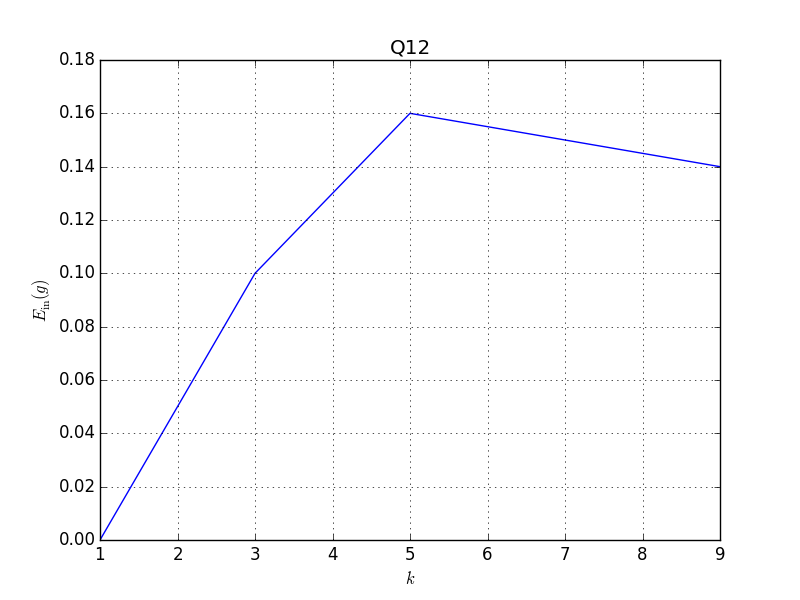
\includegraphics[scale=0.5]{Q12.png}
\end{figure}
$E_{\text{in}}\ParTh{g_{k\text{-nbor}}}$ reaches maximum at $k=5$. And $E_{\text{in}}\ParTh{g_{k\text{-nbor}}}=0$ at $k=1$, as expect.

\QEDB

\horrule{0.5pt}

\subsection*{Problem 14}

\begin{figure}[H]
	\centering
	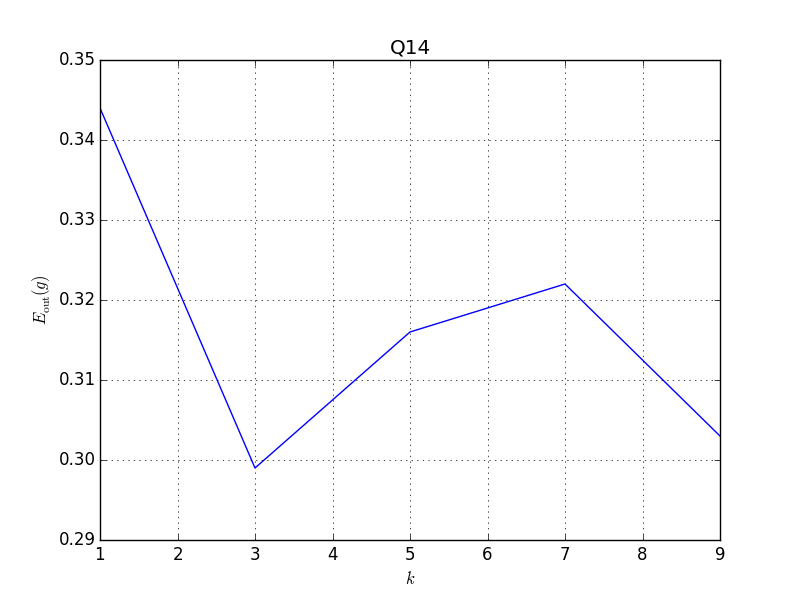
\includegraphics[scale=0.5]{Q14.png}
\end{figure}
$E_{\text{in}}\ParTh{g_{k\text{-nbor}}}$ reaches minimum at $k=3$. After $k=7$, $E_{\text{in}}\ParTh{g_{k\text{-nbor}}}$ decreases.

\QEDB

\horrule{0.5pt}

\subsection*{Problem 16}

\begin{figure}[H]
	\centering
	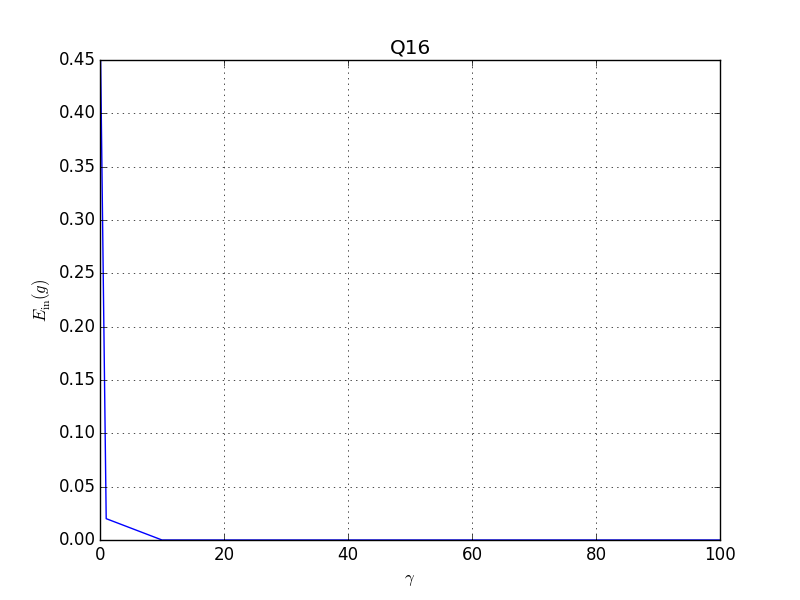
\includegraphics[scale=0.5]{Q16.png}
	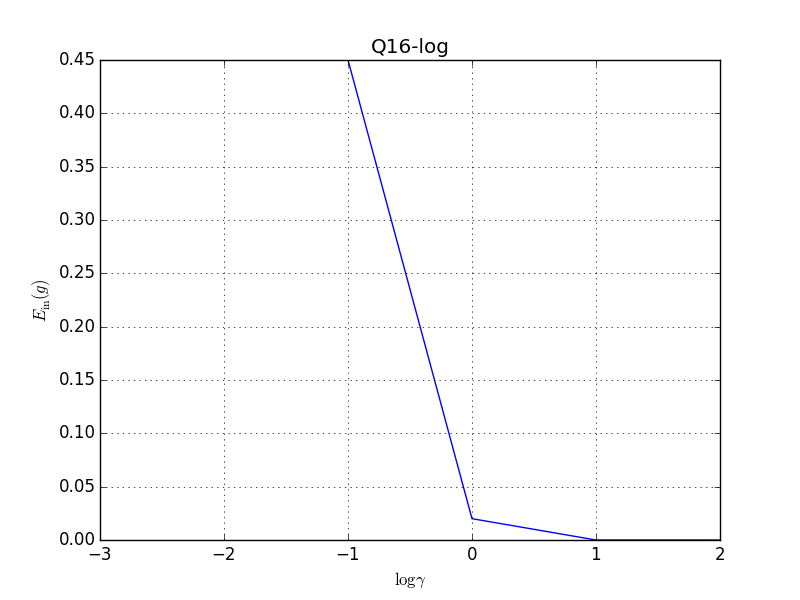
\includegraphics[scale=0.5]{Q16-log.png}
\end{figure}
As $\log\gamma>-1$, $E_{\text{in}}\ParTh{g_{\text{uniform}}}$ decreases dramatically.

\QEDB

\horrule{0.5pt}

\subsection*{Problem 18}

\begin{figure}[H]
	\centering
	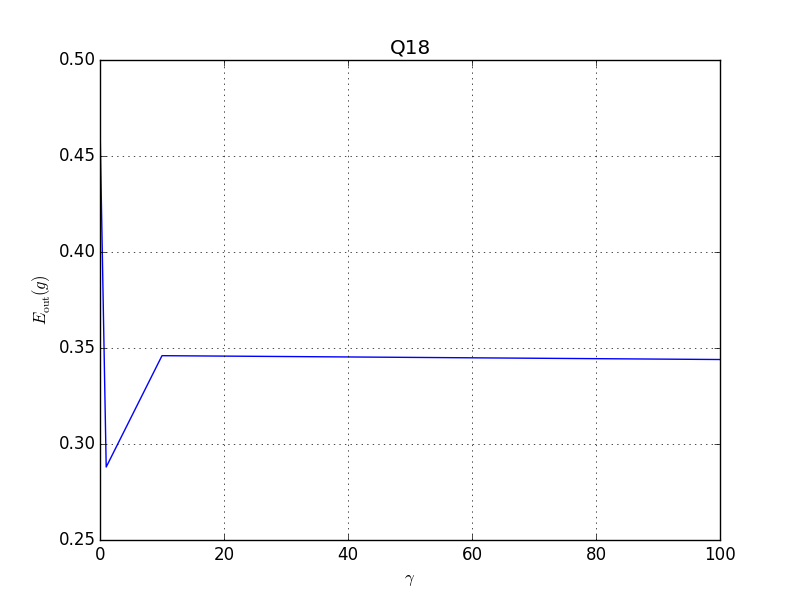
\includegraphics[scale=0.5]{Q18.png}
	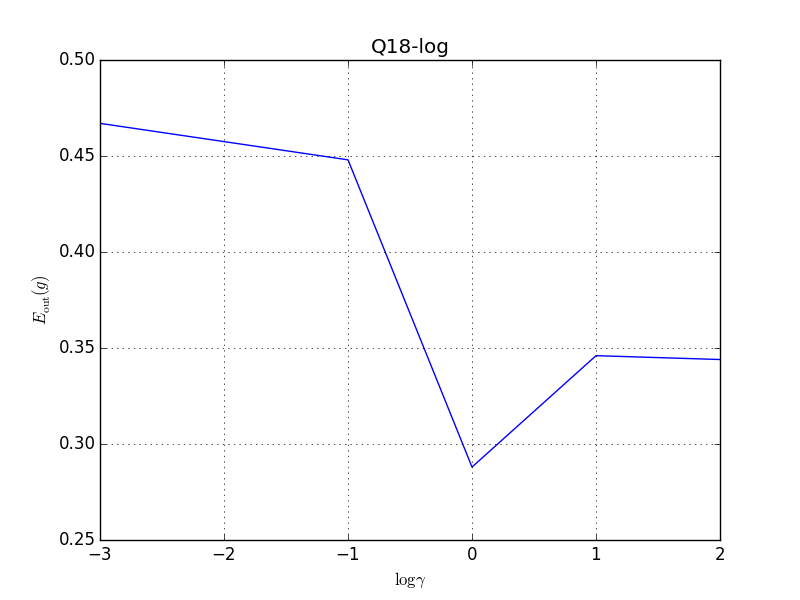
\includegraphics[scale=0.5]{Q18-log.png}
\end{figure}
As $\log\gamma=0$, $E_{\text{out}}\ParTh{g_{\text{uniform}}}$ reaches minimum and then increases. Combine the results of Problem 16, $\log\gamma>0$ may cause overfitting in this case.

\QEDB

\horrule{0.5pt}

\subsection*{Problem 20}

\begin{figure}[H]
	\centering
	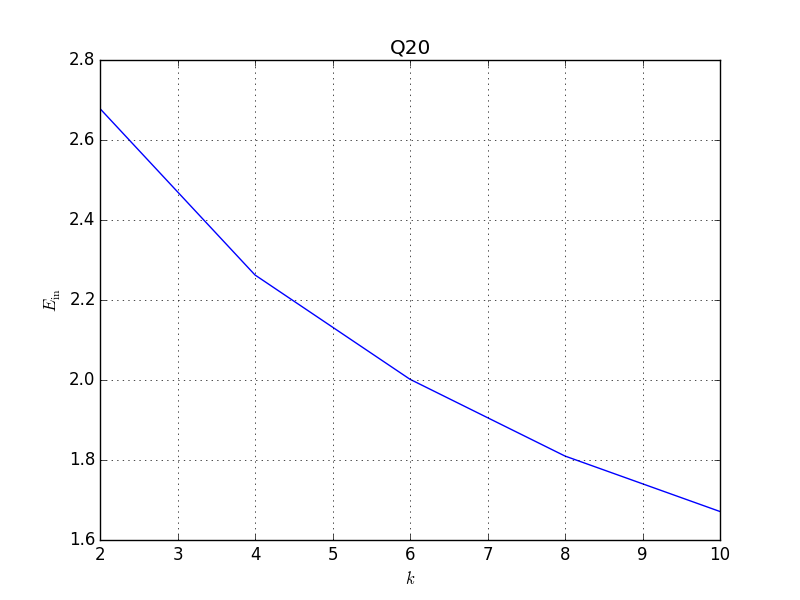
\includegraphics[scale=0.5]{Q20.png}
\end{figure}
As $k$ increases, $E_{\text{in}}$ decreases. This is reasonable since $\VecAbsVal{\BF{x}_n-\bm{\mu}_m}^2$ should be smaller if $k$ is larger.

\QEDB

\horrule{0.5pt}

\subsection*{Problem 21}

%Now we have $\Delta\geq2$ and $N\geq3\Delta\log_2\Delta\geq6$, so $2^N\geq2^6=64$ and $N^\Delta+1\geq6^2+1=37$.
For $N=\min N=3\Delta\log_2\ParTh{\Delta}$, we have the following figure
\begin{figure}[H]
	\centering
	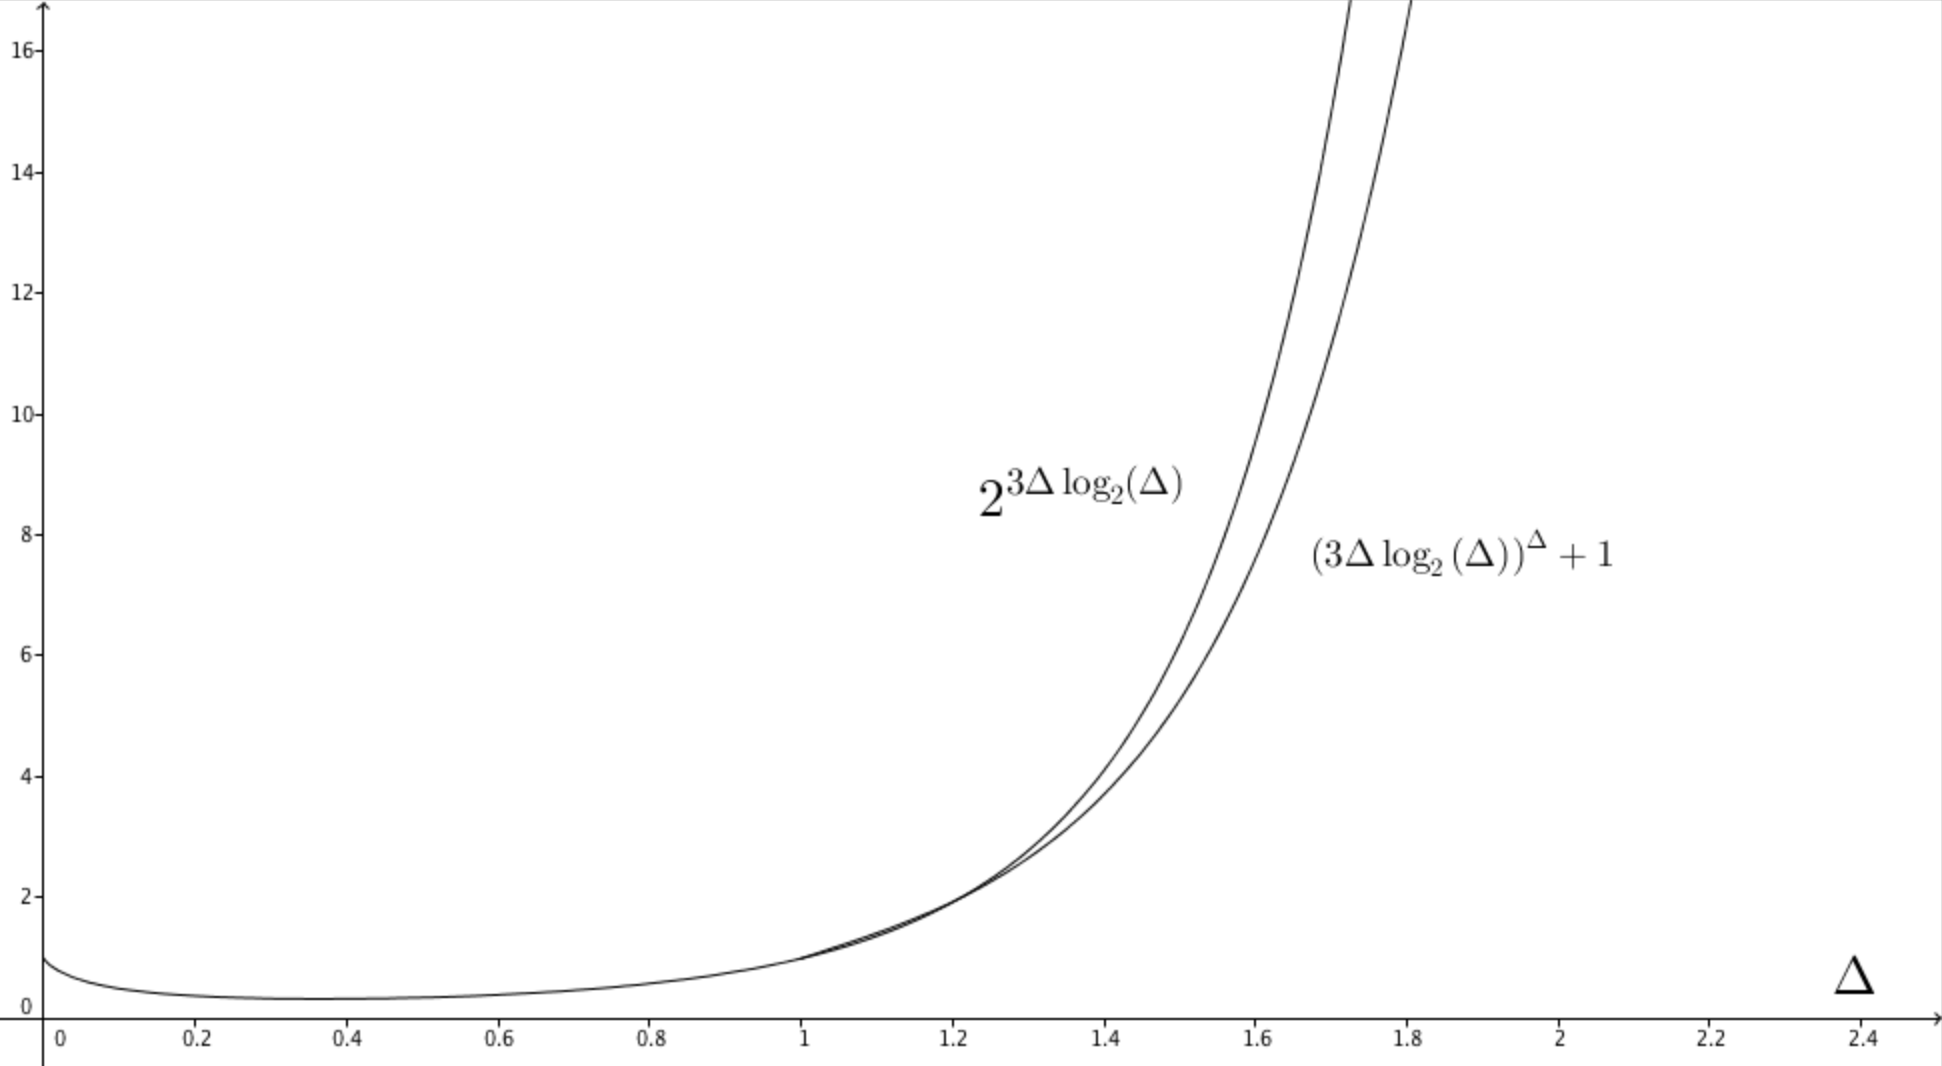
\includegraphics[scale=0.3]{21-3.png}
	\caption{$2^N$ and $N^\Delta+1$ with $N=3\Delta\log_2\ParTh{\Delta}$.}
\end{figure}
The values of $\Delta$ satisfy
\begin{align}
2^N=2^{3\Delta\log_2\ParTh{\Delta}}=\ParTh{3\Delta\log_2\ParTh{\Delta}}^\Delta+1=N^\Delta+1
\end{align}
are $\Delta=1$ and $\Delta\approx1.21033$. $\forall\Delta\geq2$, we have
\begin{align}
\ParTh{3\Delta\log_2\ParTh{\Delta}}^\Delta+1<2^{3\Delta\log_2\ParTh{\Delta}}
\end{align}
Consider some fixed $\Delta\geq2$, we have
\begin{align}
\lim\limits_{N\rightarrow\infty}\dfrac{N^\Delta+1}{2^N}=\lim\limits_{N\rightarrow\infty}\dfrac{\frac{\partial^{\lceil\Delta\rceil}}{\partial N^{\lceil\Delta\rceil}}\ParTh{N^\Delta+1}}{\frac{\partial^{\lceil\Delta\rceil}}{\partial N^{\lceil\Delta\rceil}}\ParTh{2^N}}
\end{align}
If $\Delta\in\mathbb{N}$, we have
\begin{align}
\lim\limits_{N\rightarrow\infty}\dfrac{\frac{\partial^{\lceil\Delta\rceil}}{\partial N^{\lceil\Delta\rceil}}\ParTh{N^\Delta+1}}{\frac{\partial^{\lceil\Delta\rceil}}{\partial N^{\lceil\Delta\rceil}}\ParTh{2^N}}=\lim\limits_{N\rightarrow\infty}\dfrac{\Delta!}{\ParTh{\ln\ParTh{2}}^\Delta2^N}=0
\end{align}
if $\Delta\notin\mathbb{N}$, we have
\begin{align}
\lim\limits_{N\rightarrow\infty}\dfrac{\frac{\partial^{\lceil\Delta\rceil}}{\partial N^{\lceil\Delta\rceil}}\ParTh{N^\Delta+1}}{\frac{\partial^{\lceil\Delta\rceil}}{\partial N^{\lceil\Delta\rceil}}\ParTh{2^N}}=\lim\limits_{N\rightarrow\infty}\dfrac{0}{\ParTh{\ln\ParTh{2}}^{\lceil\Delta\rceil}2^N}=0
\end{align}
This result shows that $2^N$ must be larger than $N^\Delta+1$ if $N$ is enough. Plot the figure, we have
\begin{figure}[H]
	\centering
	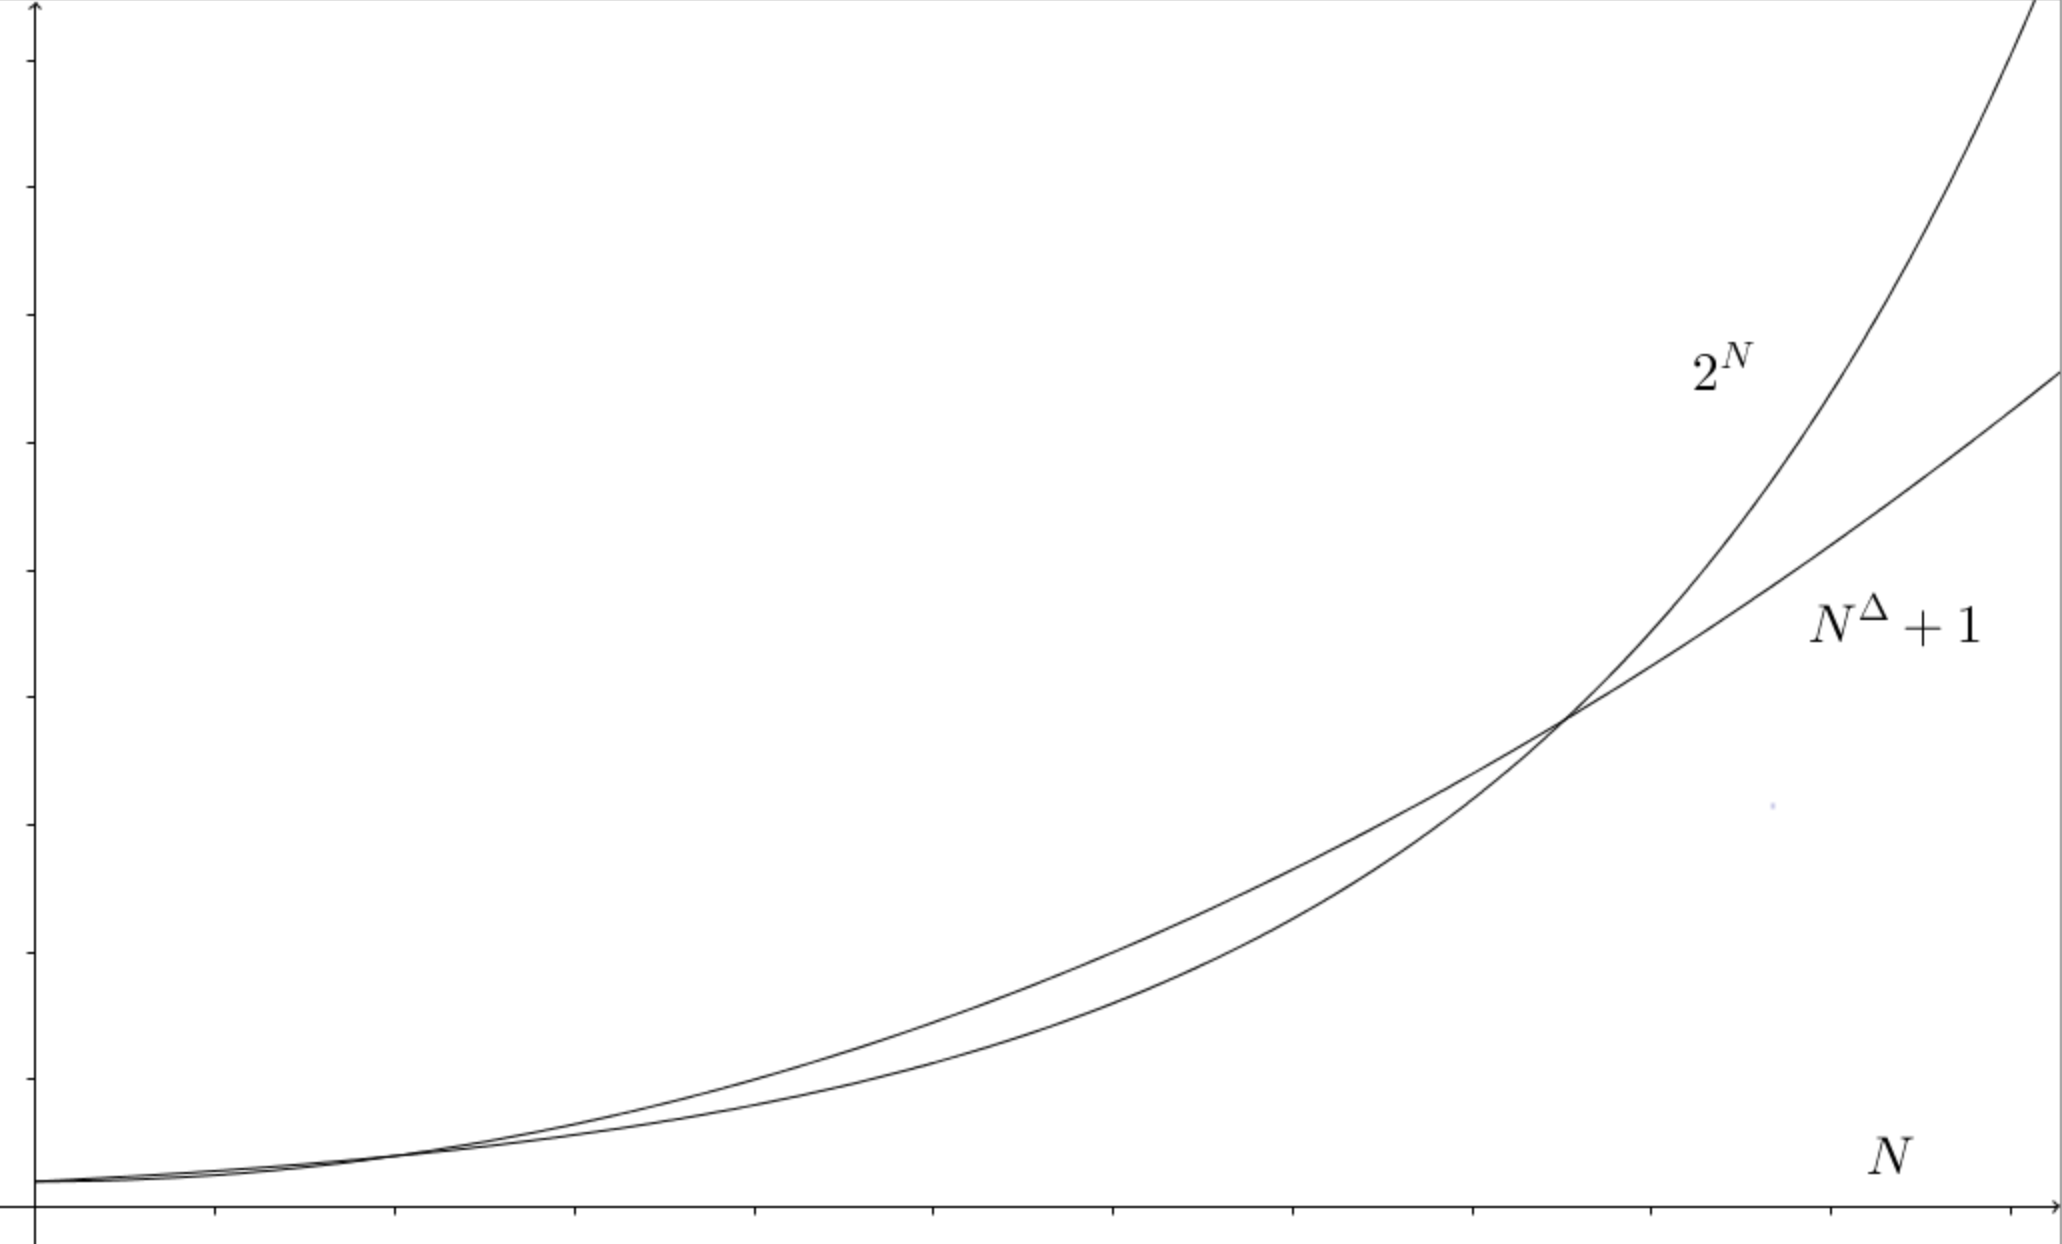
\includegraphics[scale=0.27]{21-4.png}
	\caption{$2^N$ and $N^\Delta+1$ for some fixed $\Delta$.}
\end{figure}
The values of $N$ satisfy $2^N=N^\Delta+1$ are $1$ and $f\ParTh{\Delta}$ with $f\ParTh{\Delta}>1$ and $2^N>N^\Delta+1$ if $N>f\ParTh{\Delta}$, $f\ParTh{\Delta}$ here is the ``large enough'' point for $N$.

\underline{Claim}: $f\ParTh{\Delta}\leq3\Delta\log_2\ParTh{\Delta}$.

\underline{Proof of Claim}:

Suppose by contradiction, if there exists $\Delta$ such that $f\ParTh{\Delta}>3\Delta\log_2\ParTh{\Delta}$, we have
\begin{align}
2^{3\Delta\log_2\ParTh{\Delta}} < \ParTh{3\Delta\log_2\ParTh{\Delta}}^\Delta+1\Rightarrow1<\Delta<1.21033...
\end{align}
This violates the assumption that $\Delta\geq2$. So $f\ParTh{\Delta}\leq3\Delta\log_2\ParTh{\Delta}$.

Since $N\geq3\Delta\log_2\ParTh{\Delta}\geq f\ParTh{\Delta}$, we have
\begin{align}
N^\Delta+1<2^N\text{ if }N\geq3\Delta\log_2\ParTh{\Delta},~\forall\Delta\geq2
\end{align}
\begin{comment}
\begin{align}
2^N&\geq2^{3\Delta\log_2\Delta}\geq2^{6}=64\\
N^\Delta+1&\geq\ParTh{3\Delta\log_2\Delta}^\Delta+1\geq6^2+1=37
\end{align}
and for fixed $\Delta$, we have

\begin{align}
\dfrac{\partial}{\partial\Delta}\ParTh{2^{3\Delta\log_2\Delta}}&=\ln\ParTh{2}\ParTh{3\log_2\Delta+\dfrac{3}{\ln\ParTh{2}}}2^{3\Delta\log_2\Delta}\\
\dfrac{\partial}{\partial\Delta}\ParTh{\ParTh{3\Delta\log_2\Delta}^\Delta+1}&=3\Delta^\Delta
\end{align}

\begin{align}
\dfrac{\partial}{\partial N}\ParTh{2^{N}}&=\ln\ParTh{2}2^{N}\\
\dfrac{\partial}{\partial N}\ParTh{N^\Delta+1}&=\Delta N^{\Delta-1}
\end{align}
so
\begin{align}
\dfrac{\partial_N\ParTh{2^{N}}}{\partial_N\ParTh{N^\Delta+1}}=\dfrac{\ln\ParTh{2}2^N}{\Delta N^{\Delta-1}}%\geq\dfrac{\ln\ParTh{2}2^N}{N^\Delta}\text{ since }N\geq3\Delta\log_2\Delta
\end{align}
We have
\begin{align}
\lim\limits_{N\rightarrow\infty}\dfrac{\ln\ParTh{2}2^N}{\Delta N^{\Delta-1}}=\infty
\end{align}
%Consider $2^N=N^\Delta$, we have $N=\Delta\log_2\ParTh{N}$.
which means $\ln\ParTh{2}2^N$ grows faster than $\Delta N^{\Delta-1}$ if $N$ is large. Consider $\min N=3\Delta\log_2\Delta$, we have
\begin{align}
\dfrac{\ln\ParTh{2}2^N}{\Delta N^{\Delta-1}}=\dfrac{\ln\ParTh{2}2^{3\Delta\log_2\Delta}}{\Delta\ParTh{3\Delta\log_2\Delta}^{\Delta-1}}
\end{align}
This graphs is like
\begin{figure}[H]
	\centering
	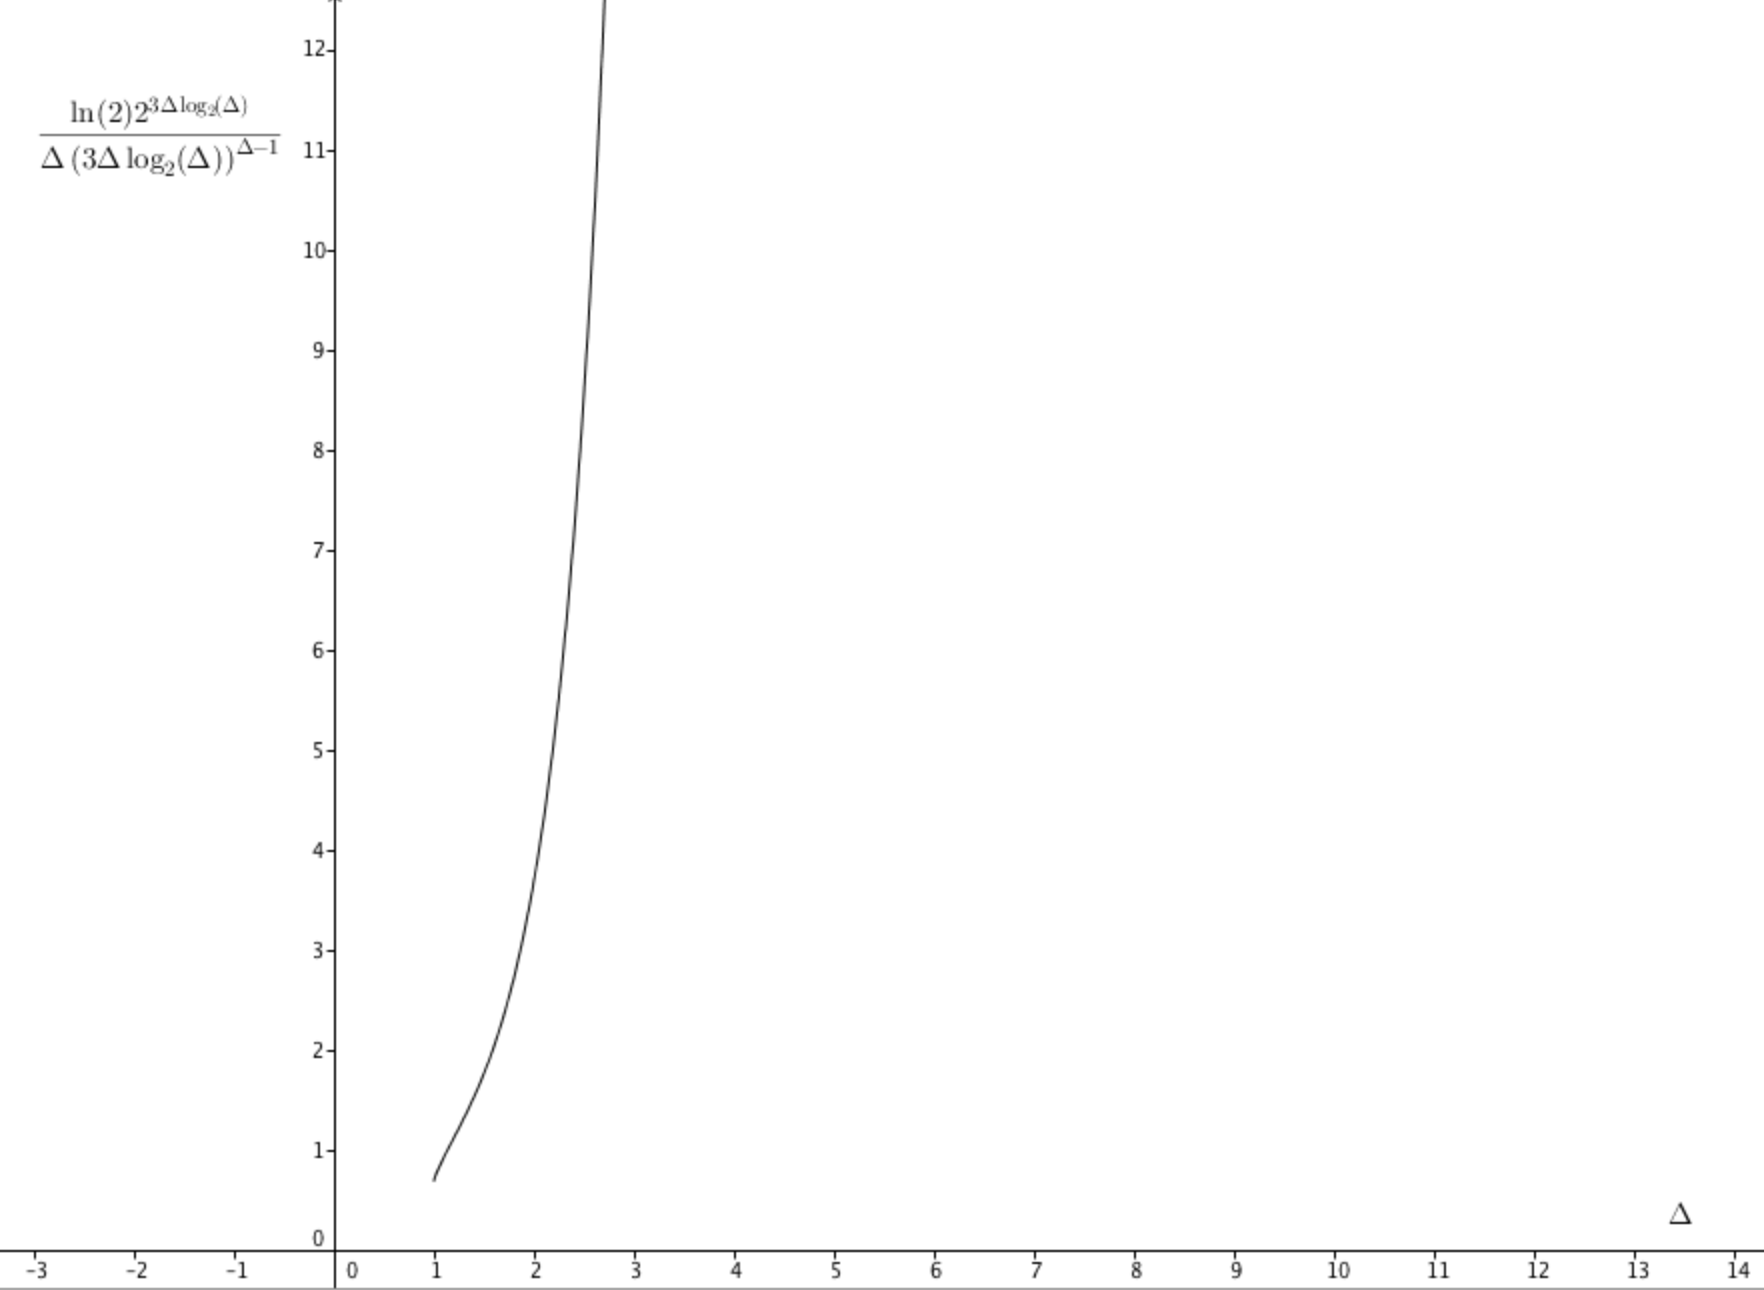
\includegraphics[scale=0.4]{21-1.png}
\end{figure}
and this function is greater than 1 for $\Delta\geq2$. For some fixed $\Delta$, we have
\begin{figure}[H]
	\centering
	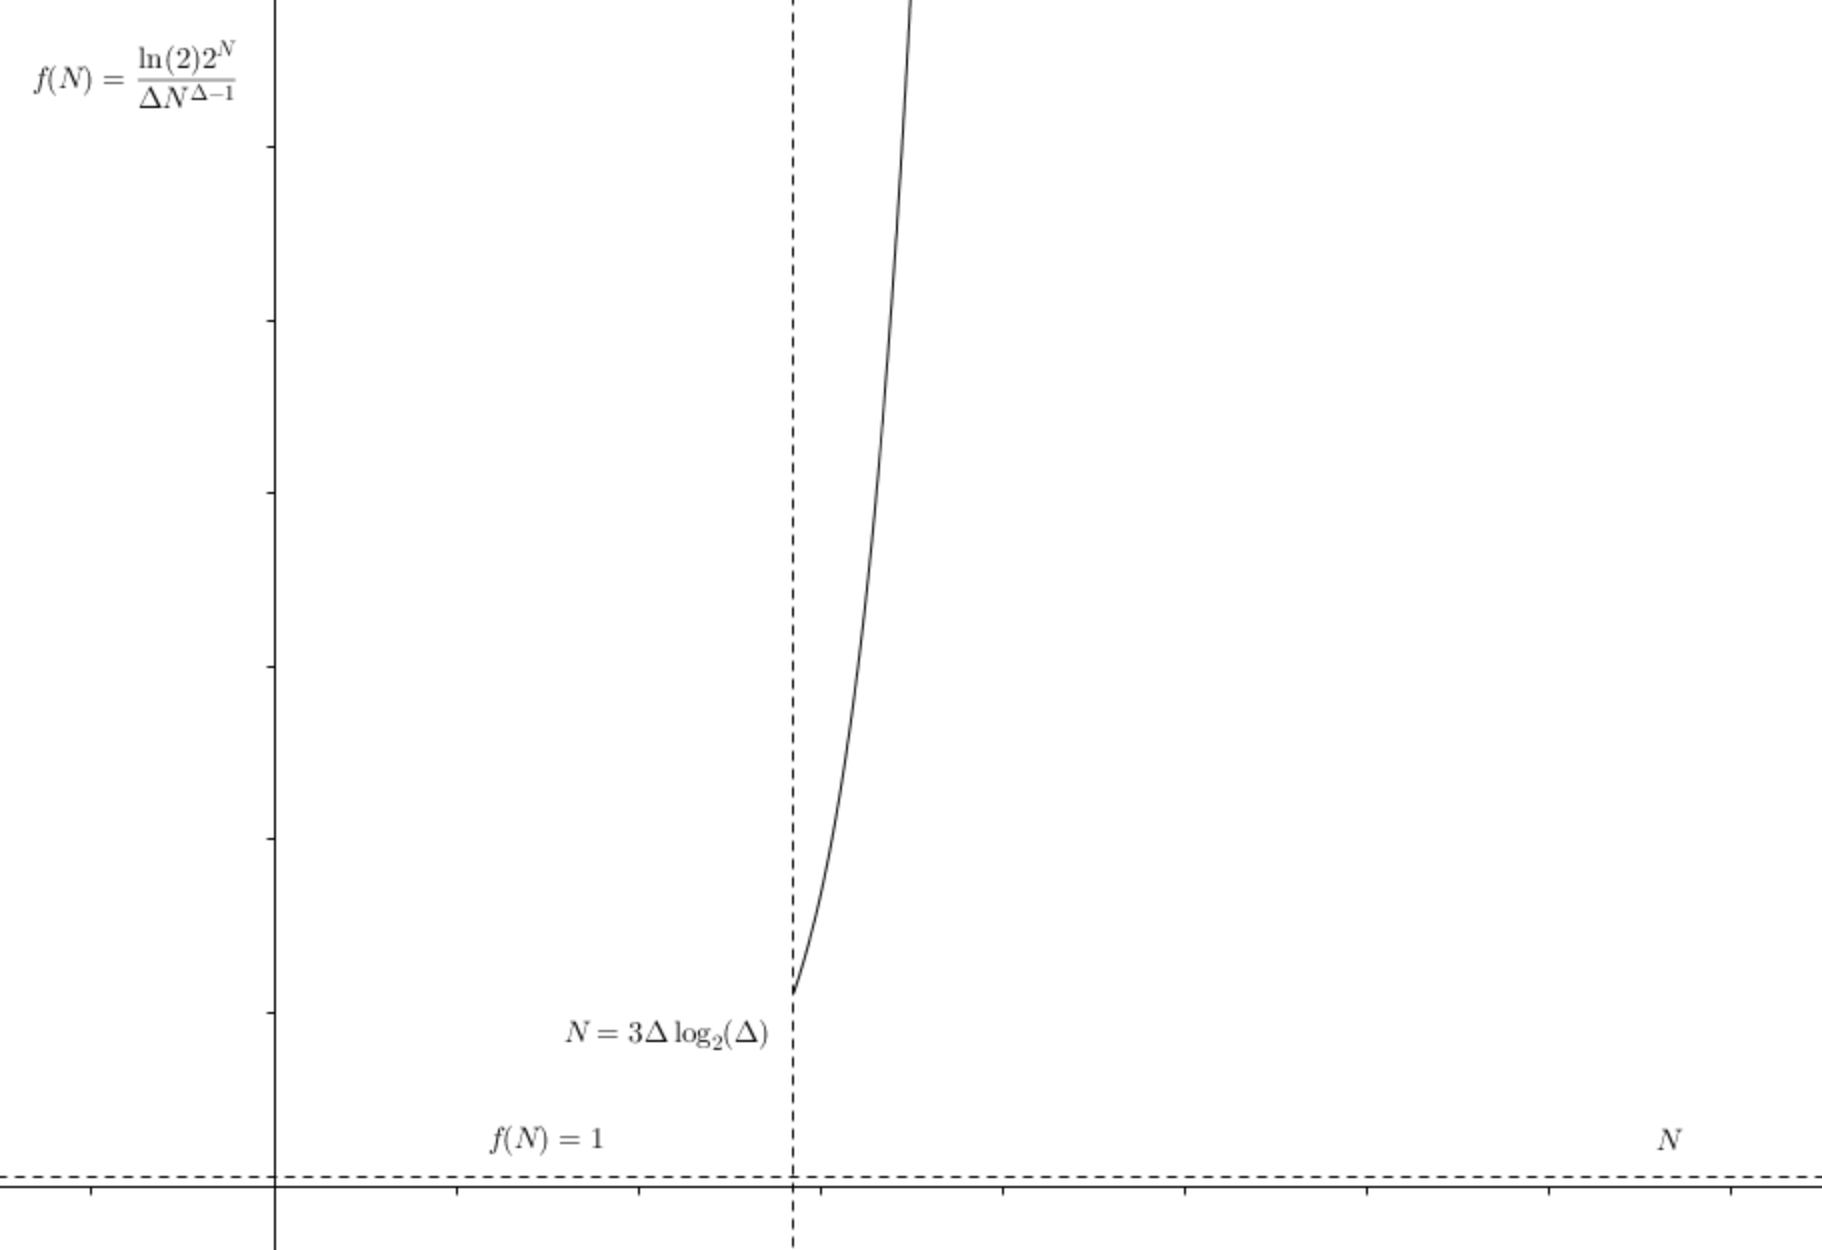
\includegraphics[scale=0.4]{21-2.png}
\end{figure}
We can see that this function is greater than 1 for $N\geq3\Delta\log_2\Delta$.

As $N$ becomes larger, $2^N$ always grows faster than $N^{\Delta}+1$ and $\min\ParTh{2^N}>\min\ParTh{N^\Delta+1}$, so $N^\Delta+1<2^N$.
\end{comment}

\QEDB

\horrule{0.5pt}

\subsection*{Problem 22}

Since $\ParTh{w^{\ParTh{2}}_{01},w^{\ParTh{2}}_{11},w^{\ParTh{2}}_{21},w^{\ParTh{2}}_{31}}=\ParTh{-2.5,1,1,1}$, the function of output layer is
\begin{align}
\text{AND}\ParTh{x^{\ParTh{1}}_1,x^{\ParTh{1}}_2,x^{\ParTh{1}}_3}
\end{align}
And we have $\ParTh{d+1}\times3=3\ParTh{d+1}$ weights between input and hidden layer. With one fixed weights of output layer, set $\Delta=3\ParTh{d+1}+1$. The VC dimension of neural network is approximately
\begin{align}
O\ParTh{\underbrace{3}_{\text{number of layers}}\times\underbrace{\ParTh{3\ParTh{d+1}+1}}_{\text{number of weights}}}
\end{align}
Set $\Delta\coloneqq3\ParTh{d+1}+1\geq2$ and $O\ParTh{3\ParTh{3\ParTh{d+1}+1}}=3\Delta f\ParTh{\Delta}$.

\underline{Claim}: $3\Delta f\ParTh{\Delta}<3\Delta\log_2\ParTh{\Delta}$.

\underline{Proof of Claim}:

Suppose by contradiction, we have
\begin{align}
3\Delta f\ParTh{\Delta}\geq3\Delta\log_2\ParTh{\Delta}
\end{align}
which means
\begin{align}
\left.m_{\mathcal{H}}\ParTh{N}\right|_{N=3\Delta\log_2\ParTh{\Delta}}=\left.2^N\right|_{N=3\Delta\log_2\ParTh{\Delta}}=2^{3\Delta\log_2\ParTh{\Delta}}
\end{align}
This is a contradiction since $m_{\mathcal{H}}\ParTh{N}\propto N^d$ and from the conclusion of Problem 21,
\begin{align}
N^d<N^\Delta+1<2^N
\end{align}
Hence, we have $3\Delta f\ParTh{\Delta}<3\Delta\log_2\ParTh{\Delta}$.

\QEDB

\horrule{0.5pt}

\section*{Reference}

\begin{enumerate}

\item[{[1]}] Lecture Notes by Hsuan-Tien LIN, Department of Computer Science and Information Engineering, National Taiwan University, Taipei 106, Taiwan.

\end{enumerate}

\end{document}